% !TEX root = ../Dokumentation.tex
\subsection{Intelligente Systeme}

\subsubsection{Softwarekonzept}
Das Softwarekonzept basiert auf dem MVC\footnote{MVC = Model-View-Control}-Prinzip, wobei sich die View auf einen reinen Debug-Zweck beschränkt. Der Controller kommunziert mit allen Subprozesse und grenzt an die Schnittstelle zur Hardwaresteuerung. Um die Performance des Rasperry Pi möglichst auszunutzen wird mit Threads gearbeitet. Die parallel laufenden Subprozesse sind:

\begin{itemize}
\item Bilderzeugung,
\item Objekterkennung und
\item Fahrbahnerkennung.
\end{itemize}

\begin{figure}[H]
	\centering
	\includegraphics[width=0.8\textwidth]{03_Loesungskonzept/pictures/grobablauf.png}
	\caption{Aktivitätendiagramm Grobablauf}
\end{figure}

Der Zustand des Fahrzeuges wird im Model gespeichert und steht allen Prozessen zur Verfügung. Die Datenstruktur ist dabei so aufgebaut, dass keine Zugriffskonflikte entstehen sollten.\\
Der Controller behandelt alle Anweisungen der Prozesse. Meldet beispielsweise die Objekterkennung einen Container, hat dieser Priorität vor dem normalen Fahren und das Mikrocontroller-Board erhält die entsprechenden Anweisungen. Das folgende Diagramm zeigt eine Gesamtübersicht von den verschiedenen Komponenten.\\[0.2cm]
\begin{figure}[H]
\centering
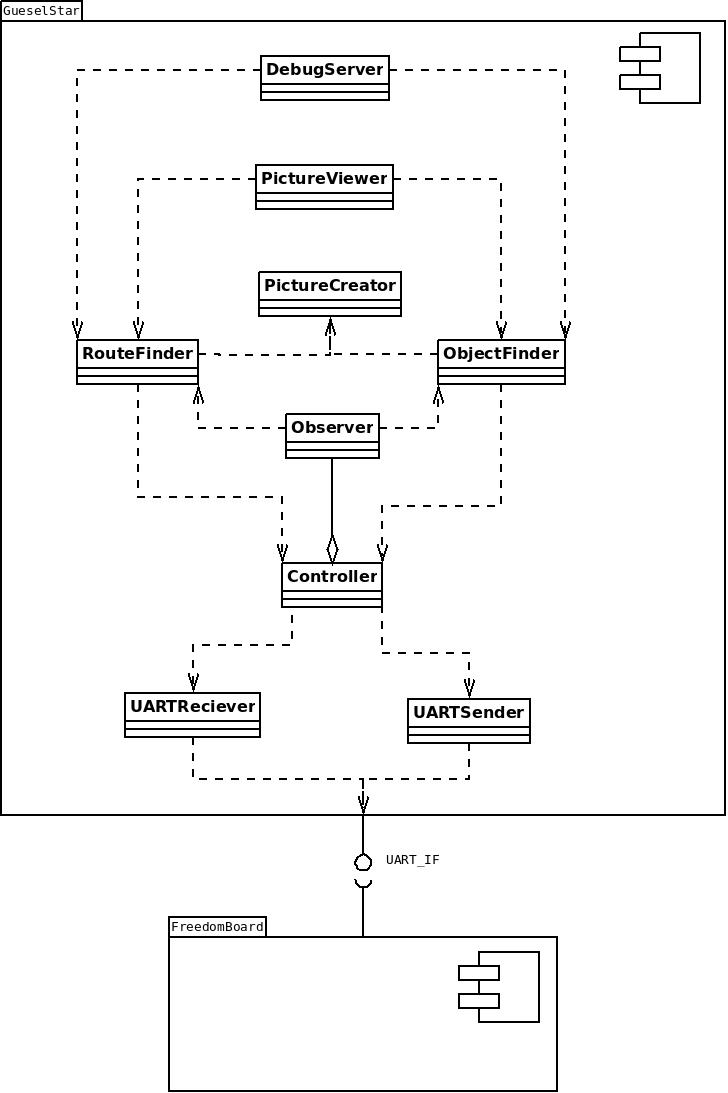
\includegraphics[width=0.8\textwidth]{03_Loesungskonzept/pictures/Komponentendiagramm_detailliert_v2.jpeg}
\caption{Komponentendiagramm}
\end{figure}

\textbf{Debug-View}\\[0.2cm]
Um während der Implementierungs-Phase der geschriebene Code zu testen wurde eine Debug-View entwickelt. Mit dieser kann auf den Debug-Server, welcher auf dem Raspberry Pi gestartet wird, zugegriffen werden. Nach einer erfolgreichen Verbindung werden die aufgenommenen Bilder vom Server an den Client (GueselStarObserver) gesendet.

\begin{figure}[H]
\centering
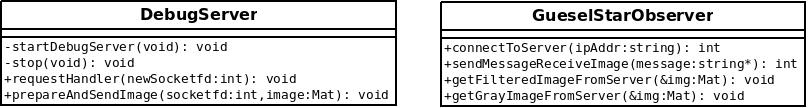
\includegraphics[width=0.8\textwidth]{03_Loesungskonzept/pictures/DebugView.jpeg}
\caption{Debug-View}
\end{figure}

Die Kommunikation zwischen Server und Client läuft über TCP/IP. Auf dem Server wird ein Server-Socket geöffnet, auf welches sich der Client verbinden kann.

\textbf{Konfiguration}\\[0.2cm]
Neu geschriebener Code benötigt einen erneuten Build. Um einen neuen Build, welcher Zeit benötigt, zu unterbinden wurde eine Konfigurations-Datei erstellt, in welcher alle benötigten Parameter angepasst werden können. Das Einlesen der Konfiguration erfolgt über einen selbstentwickelten Parser und wird anschliessend in einem Objekt der Klasse "PRENConfiguration" abgespeichert.

\begin{figure}[H]
\centering
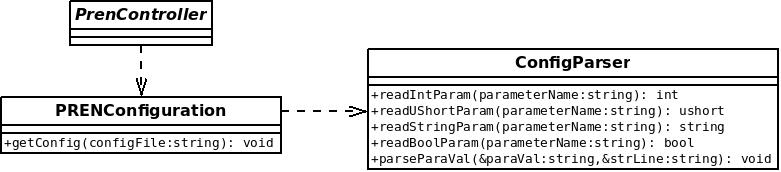
\includegraphics[width=0.8\textwidth]{03_Loesungskonzept/pictures/Configuration.jpeg}
\caption{Konfiguration}
\end{figure}
 
%***************************
\subsubsection{Mikrocontroller-Board}
\textbf{Funktionsbeschrieb}\\[0.2cm]
Das Mikrocontrollerboard bildet die Schnittstelle zwischen der Hardware (Motoren und Sensoren) und dem Minicomputer. Das Mikrocontrollerboard übernimmt die Ansteuerung und Auswertung der einzelnen Komponenten und stellt die verarbeiteten Informationen dem Minicomputer über eine Schnittstelle zur Verfügung.\\[0.2cm]
\newpage
\textbf{Komponentenbeschrieb}
\begin{figure}[H]
	\centering
	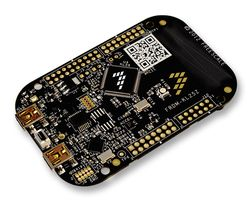
\includegraphics[width=0.45\textwidth]{03_Loesungskonzept/pictures/freedomboard.png}
	\caption{Freedomboard KL25 von Freescale (Quelle:http://ch.farnell.com/)}
	%http://ch.farnell.com/productimages/standard/de_DE/freescalesemiconductor-frdm-kl25z-40.jpg
\end{figure}
Als Mikrocontrollersystem wurde das Freedomboard KL25Z von Freescale ausgewählt. Das Entwicklungsgsboard bietet vieles, wie ausreichend I/O's, AD Wandler und Timerausgänge. Das Board wird mit der Programmiersprache C programmiert.\\[0.2cm]
\textbf{Begründung}\\[0.2cm]
Das Board überzeugt durch eine gute Rechenperformance zu einem kleinen Preis. Das Hauptargument für das Freedomboard ist die einfache Programmierung. Für viele Komponenten wie Servos oder Ultraschalsensoren steht ein Tool namens ProcessorExpert zu Verfügung. Dieses Tool ermöglicht eine relativ einfache Anbindung solcher Komponenten. Dies spart sehr viel Entwicklungsaufwand.
Das Freedomboard hat sich gegen das Tinkerforgesystem durchgesetzt. Der Hauptgrund ist die Flexibilität des Freedomboards gegenüber dem Tinkerforgesystem. Dieses ist sehr einfach zu bedienen solange alle Komponenten von Tinkerforge zur Verfügung gestellt werden. Fehlt aber ein Modul wird es sehr schnell kompliziert. Beim Freedomboard ist der Aufwand für eine Komponente etwas höher, dafür können die meisten Systeme angeschlossen werden.\\[0.2cm]
\textbf{Testergebnisse}\\[0.2cm]
Das Freedomboard wurde als Funktionsmuster bereits in Betrieb genommen. Es hat sich gezeigt, dass die Anbindung der Komponenten tatsächlich sehr einfach ist. Es wurden bereits ein Ultraschallsensor, mehrere Servos, eine UART Kommunikation und ein Infrarotsensor angebunden. Das System lieferte dabei sehr vielversprechende Ergebnisse.\\[0.2cm]
\textbf{Software Grundaufbau}\\[0.2cm]
Das Tool ProcessorExpert bietet eine Komponente FreeRTOS an. Das ist ein Betriebssystem, welches das Programmieren sehr vereinfacht. Damit können verschiedene Tasks definiert werden und quasi parallel ausgeführt werden. Die Software wird damit geplant. Folgende Tasks sind geplant:
\begin{figure}[H]
	\centering
	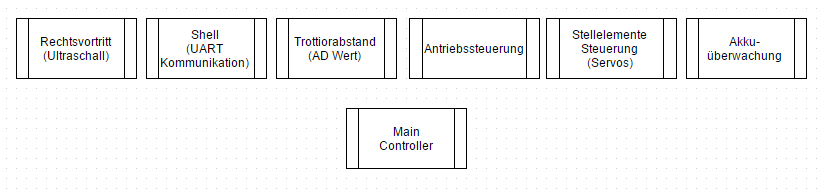
\includegraphics[width=0.9\textwidth]{03_Loesungskonzept/pictures/MC_Tasks.png}
	\caption{Übersicht MC Tasks}
\end{figure}
Die Implementierung der Tasks wird im Modul Produkteentwicklung zwei (PREN2) umgesetzt.